%% ===========================================================================
%% From Fuel Customers to Flight Geography: aviation emissions for Pakistan
%% Target journal: Environmental Modelling & Software (Elsevier)
%% ===========================================================================
\documentclass[5p,times,authoryear]{elsarticle}
% ===========================================================================
% Shared preamble for every manuscript in this repository.
%
% Papers using it:
%   paper/            agriculture inventory
%   paper_nowcast/    agricultural nowcasting
%   paper_national/   the nine-sector national inventory
%   notes/<sector>/   one data note per non-agriculture sector
%
% It exists because paper/ and paper_nowcast/ began as copies of one another
% and had already drifted five lines apart before a third manuscript existed.
% Eleven copies would drift eleven ways, and a macro that renders differently
% in two papers is the kind of defect nobody notices until proof stage.
%
% \graphicspath is deliberately NOT set here - each manuscript sets its own
% after \input{...preamble}, because figures live beside the document.
% ===========================================================================

\usepackage[utf8]{inputenc}
\usepackage[T1]{fontenc}
\usepackage{amsmath,amssymb}
\usepackage{graphicx}
\usepackage{booktabs}
\usepackage{multirow}
\usepackage{siunitx}
\usepackage[colorlinks=true,citecolor=blue,linkcolor=blue,urlcolor=blue]{hyperref}
% Document-information metadata for every PDF in the bundle (the seventh review noted
% the shipped PDFs carried none). Documents that set their own \hypersetup{pdftitle=...}
% keep it - hyperref takes the LAST setting, and this shared block runs first. Full
% tagged-PDF (tagpdf / \DocumentMetadata) is deliberately not attempted here: the
% installed LaTeX toolchain's support is not uniform across sixteen documents, and a
% half-tagged bundle is worse than an honestly untagged one; deferred deliberately.
\hypersetup{
  pdfauthor={Rehan Ahmad, Pakistan Air Quality Initiative (PAQI)},
  pdfsubject={A reproducible ten-sector national greenhouse-gas inventory
              for Pakistan},
  pdfkeywords={Pakistan, greenhouse gas inventory, IPCC 2006 Guidelines, MRV,
               reproducible research, emissions, air pollutants},
}
\usepackage{caption}
\captionsetup[table]{position=below}
\usepackage{enumitem}
\usepackage{xcolor}
\usepackage{float}
\usepackage{placeins}
\usepackage{tabularx}
\usepackage{natbib}
\usepackage{tikz}
\usetikzlibrary{arrows.meta,positioning,fit,backgrounds}

\setlength{\emergencystretch}{3em}

% Looser float placement to prevent pile-up in two-column mode.
\renewcommand{\topfraction}{0.95}
\renewcommand{\bottomfraction}{0.85}
\renewcommand{\textfraction}{0.05}
\renewcommand{\floatpagefraction}{0.85}
\setcounter{topnumber}{4}
\setcounter{bottomnumber}{3}
\setcounter{totalnumber}{6}

% ---------------------------------------------------------------------------
% Custom shorthand: in macros.tex since the ESSD re-targeting, because the national
% article compiles under the Copernicus class and cannot take this preamble (the class
% loads its own packages) but needs exactly the same macros. This file inputs it so that
% every other manuscript keeps compiling unchanged.
%
% THREE relative paths, because \input resolves against the COMPILE DIRECTORY and not
% against this file, so the depth is a property of whoever is building:
%   ../paper_common      a manuscript compiled from one level down
%   ../../paper_common   papers/<sector>/ and notes/<sector>/
%   ../../../paper_common  paper_national/versions/<v>/, since the national paper was
%                          versioned - that move is what added this third arm, and the
%                          supplement failed with "../../paper_common/macros.tex not
%                          found" until it was here
% A fourth depth needs a fourth arm, which is the cost of keeping a bare `latexmk` in a
% manuscript directory working without a TEXINPUTS set for it.
% ---------------------------------------------------------------------------
\IfFileExists{../paper_common/macros.tex}%
  {\input{../paper_common/macros}}%
  {\IfFileExists{../../paper_common/macros.tex}%
    {% ===========================================================================
% paper_common/macros.tex - the shorthand every manuscript shares.
%
% Split from preamble.tex in the ESSD re-targeting: the national article now compiles
% under the Copernicus class, which loads its own packages and forbids most of what
% preamble.tex sets (geometry-like options, a second hyperref, placeins), but it needs
% exactly the same shorthand as the sector reports. The macros therefore live here, on
% their own, and preamble.tex inputs this file so that every other manuscript keeps
% compiling unchanged. A macro that renders differently in two documents is the defect
% this file exists to prevent; define it once.
%
% Requires: siunitx (for \DeclareSIUnit and \si) - the caller loads it.
% ===========================================================================

% Gas and pollutant names.
\newcommand{\COtwo}{CO\textsubscript{2}}
\newcommand{\COe}{CO\textsubscript{2}e}
\newcommand{\CHfour}{CH\textsubscript{4}}
\newcommand{\NtwoO}{N\textsubscript{2}O}
\newcommand{\NHthree}{NH\textsubscript{3}}
\newcommand{\NOx}{NO\textsubscript{x}}
\newcommand{\SOtwo}{SO\textsubscript{2}}
\newcommand{\PM}{PM\textsubscript{2.5}}
\newcommand{\MCF}{MCF}
\newcommand{\Mt}{\text{Mt~\COe}}
\newcommand{\tCha}{\si{\tonne\per\hectare}}
\newcommand{\AFOLU}{AFOLU}
\newcommand{\GLW}{GLW\,4}
\newcommand{\EFone}{EF\textsubscript{1}}

% siunitx: allow Mt, Tg, ha, head, yr, dB
\DeclareSIUnit{\head}{head}
\DeclareSIUnit{\yr}{yr}
\DeclareSIUnit{\dB}{dB}

% A file name is the one long unbreakable token these documents are full of -
% \texttt{waste\_air\_pollutants\_2024.csv} is wider than a two-column measure and TeX prints
% it past the margin rather than breaking it. Allowing a break AFTER each escaped underscore
% costs nothing and inserts no hyphen, which matters: a hyphenated file name is a wrong file
% name. This is one line because every such name in every document is written with \_.
\let\pkinvunderscore\_
\renewcommand{\_}{\pkinvunderscore\allowbreak}
}%
    {\input{../../../paper_common/macros}}}
% Long unbreakable strings - output filenames, module paths, URLs in \texttt - do not fit a
% two-column measure and TeX prints them past the margin rather than breaking them. Nothing
% read the log, so 47 of those overruns shipped across seven documents. Emergency stretch lets
% the paragraph loosen instead, and \texttt is taught to break at the punctuation these names
% actually contain.
\emergencystretch=6em


\graphicspath{{figures/}}
\journal{Environmental Modelling \& Software}
\begin{document}
\begin{frontmatter}
\title{PakEmis Sector Technical Note TN10\\[4pt]
From Fuel Customers to Flight Geography: A Reproducible Aviation Emissions Account for Pakistan}
\author[paqi]{Rehan Ahmad\corref{cor1}}
\ead{rehan@pakairquality.com}
\address[paqi]{Pakistan Air Quality Initiative (PAQI), Karachi, Pakistan}
\cortext[cor1]{Corresponding author}
\begin{abstract}
Petroleum statistics classify aviation fuel by customer, whereas greenhouse-gas inventories
classify flights by origin and destination. We develop a source-row-conserving bridge between
these systems for Pakistan using annual fuel reports, five matched fiscal years of OECD
aviation estimates and 42 monthly comparisons. In FY2023--24, commercial aviation fuel implies
\SI{2.032}{\mega\tonne} \COtwo{}, 0.8\% below OECD's combined domestic and international
territory estimate. This aggregate agreement is misleading: resident-customer fuel is 28.6\%
above OECD's resident-carrier estimate, while foreign-customer fuel is 23.1\% below its
non-resident estimate, causing 97\% of the component discrepancy to cancel.

The figure the national inventory carries is the aggregate movement model's
\SI{0.301}{\mega\tonne} \COe{} (0.299 Mt as \COtwo{} alone) --- the estimator with the
strongest activity evidence behind it, and the one every national product uses. Around it:
the OECD resident-carrier partition gives \SI{0.292}{\mega\tonne} of domestic \COtwo{},
which is a calibrated consistency check rather than independent validation because OECD
supplies that partition, and the route--aircraft Monte Carlo gives a mean of 0.244 Mt
\COtwo{} with a 95\% interval of 0.215--0.272 Mt. Pakistan's official 2022 reporting instead applies an 80/20
domestic--international allocation that is not consistent with the petroleum and
flight-geography evidence examined here. The framework conserves every reported fuel row,
keeps unresolved quantities explicit and separates calibration, external evaluation,
structural uncertainty and parametric uncertainty. It provides a transferable method for
reconciling purchaser-based petroleum statistics with flight-based aviation accounts.

The common annual core now reaches FY2024--25. Its LTO allocation uses the corresponding complete PCAA airport-movement source, with the reference aircraft composition explicitly carried where own-year fleet evidence is absent. The detailed route, OECD and structural comparisons in this note remain anchored to FY2023--24.

\end{abstract}
\begin{keyword}
civil aviation \sep fuel reconciliation \sep flight geography \sep international bunkers \sep
structural uncertainty \sep IPCC 2006 Guidelines \sep Pakistan
\end{keyword}
\end{frontmatter}

%% Generated by scripts/make_release_cover.py; says which release this documents.
% The Sector Technical Note banner (v1.0.0). Each sector manuscript is a PakEmis Sector
% Technical Note, numbered TN01-TN10 in src/pkinv/release.py (TECHNICAL_NOTES), and says
% so on its first page: it documents ONE sector module of the release named in the block
% that follows, and the national totals are stated only in the data-description article
% (the cover block below reproduces them as release identity, not as a claim of this note).
% Usage, in the document body before the release cover:  \TNBanner{TN01}
\providecommand{\TNBanner}[1]{%
  \noindent\fbox{\parbox{\dimexpr\linewidth-2\fboxsep-2\fboxrule}{%
    \textbf{PakEmis Sector Technical Note #1.} Technical documentation of one sector
    module of the PakEmis release identified below, deposited with the data as part of the
    documentation record. The national data-description article (\texttt{paper\_national/})
    is the only document that states the national totals as its own result.%
    \InputIfFileExists{../../paper_common/generated_availability_tn}{}{}%
  }}\par\medskip}

\TNBanner{TN10}
%% GENERATED by scripts/make_release_cover.py from outputs/release_manifest.json.
%% Do not edit: the edit will be overwritten and CI diffs the result.
\newcommand{\ReleaseCover}{%
\begin{center}\small
\setlength{\fboxsep}{4pt}%
\fbox{\begin{minipage}{\dimexpr\linewidth-2\fboxsep-2\fboxrule\relax}\footnotesize
\textbf{Release provenance.} This document describes PakEmis under the period, configuration and source boundaries specified in its methods. The identifiers below link it to the accompanying products and source register.\\[2pt]
\begin{tabular}{@{}p{0.32\linewidth}@{\hspace{0.03\linewidth}}p{0.65\linewidth}@{}}
Release version & \texttt{1.0.0rc69} \\
Commit & \texttt{d8d874622f9a} \\
Reporting period & July 2015--June 2025 (ten fiscal years) (2015-07-01 to 2025-06-30) \\
Reference & S\_TAN (household survey; TAN nitrogen) \\
FY2023--24 total & 444.61 Mt \COe{} (AR5) under S\_TAN, the reference; 449.85 Mt under L\_TAN \\
Release manifest & \texttt{ac0ffe93ad9fcd88} (SHA-256 of \texttt{outputs/release\_manifest.json}, first 16) \\
Source manifest & \texttt{c1be6d314cfce1ea} (SHA-256 of \texttt{data/manifests/source\_manifest.csv}, first 16) \\
Data-description article & \texttt{paper\_national/} (ESSD, in preparation), same release
\end{tabular}
\end{minipage}}
\end{center}}

\ReleaseCover

\section{Introduction}
\label{sec:introduction}

National aviation accounts must distinguish three concepts: who bought the fuel, which carrier
operated the aircraft and whether a flight stage was domestic or international. Petroleum
statistics commonly follow purchasers. IPCC inventories instead classify each flight from its
origin and destination, irrespective of airline nationality \citep{ipcc2006energy}. A national
airline can therefore buy fuel recorded under a domestic customer label while using much of it
on international services.

Pakistan makes the consequences visible. A movement-based calculation placed domestic
aviation near \SI{0.30}{\mega\tonne} \COe{} in FY2023--24, but had no fuel control and carried
a broad representation uncertainty. Public Oil Companies Advisory Council (OCAC) statistics
report JP-1 separately for PIA, other Pakistani-airline customers and foreign aviation. Read
literally, the resident-customer rows imply almost four times the movement estimate. That is
not evidence of fourfold domestic emissions: ``Domestic Avi--PIA'' identifies a purchaser, not
a domestic flight boundary.

The problem is a conserved partition rather than another uncertain percentage. Reassigning a
tonne from domestic aviation also changes international bunkers or another aviation account.
The source row must therefore remain intact while its destinations, method and unresolved
quantity stay visible. A second distinction follows. OECD estimates monthly territory- and
residence-based aviation emissions from flight data \citep{oecdaviation}. Those data can help
partition resident-customer fuel, but an estimate produced with that partition cannot then be
presented as an independent OECD validation. Gross fuel and flight accounts can still be
compared more independently, and their resident and foreign components can reveal whether an
apparently good total is internally coherent.

Aircraft-performance detail addresses a different layer. ICAO route factors and OpenAP
synthetic profiles can test the consequences of representative distance, route mix and
aircraft assignment \citep{icaoicec2024,sun2020openap}. Climate TRACE provides an additional
airport-level comparison, although surveillance and performance inputs may overlap with other
flight models \citep{climatetrace}. These sources strengthen the evidence hierarchy only when
their roles and shared inputs are declared in advance.

We therefore ask one question: can purchaser-based aviation-fuel statistics be reconciled with
flight-geography accounts without allowing aggregate agreement to conceal errors in the
underlying components? We answer it with nine OCAC fuel years, five complete fiscal-year OECD
comparisons, 42 matched months, Pakistan's official UNFCCC reporting and a hierarchy of
domestic activity models.

The paper makes three contributions. First, it introduces a source-row-conserving bridge that
separates purchaser, carrier residence and flight geography across domestic aviation,
international bunkers, military/government, general aviation, other uses and an explicit
residual. Second, it shows that near-closure of Pakistan's gross commercial aviation account
conceals persistent resident and foreign discrepancies of opposite sign. Third, it evaluates
domestic aviation through aggregate-movement, route-resolved and route--aircraft estimates,
with calibration, external comparison, structural scenarios and parametric uncertainty kept
distinct. Movement-to-cycle conversion, flight-geography classification and full-flight fuel
remain executable accounting safeguards rather than headline contributions.

\section{Data and Accounting Boundaries}
\label{sec:data}

Pakistan Civil Aviation Authority (PCAA) statistics provide the activity controls. The
FY2023--24 airport report records 40,600 domestic and 95,267 international commercial
movements, 21,223 non-commercial movements and 5.680 million domestic passengers
\citep{pcaaairports2024}. A separate airline report gives departures, arrivals, passengers,
cargo and mail by operator \citep{pcaaairlines2024}. One movement is one take-off or landing;
the national domestic activity control is therefore 20,300 flight stages. The historical
movement series covers FY2006--07 to FY2023--24.

OCAC sectoral reports provide the fuel control. In FY2023--24 they record
\SI{193813}{\tonne} of JP-1 for ``Domestic Avi--PIA'', \SI{166119}{\tonne} for ``Domestic
Avi--Others'' and \SI{283147}{\tonne} for ``Overseas/Foreign Aviation'', with government
JP-1, JP-8 and 100LL retained separately \citep{ocacaviation}. Final reports supply nine annual
fuel accounts from FY2016--17 to FY2024--25; public cumulative reports supply 42 months that
overlap OECD completely. Revisions and category-label changes are versioned rather than
silently harmonised \citep{ocacarchive}.

OECD monthly aviation estimates cover calendar 2019--2024 and distinguish domestic and
international territory emissions from resident- and non-resident-carrier activity
\citep{oecdaviation}. In FY2023--24 they report 235.8 kt \COtwo{} for domestic territory
aviation and 1812.0 kt for international aviation. Resident carriers account for 227.0 kt of
domestic and 657.3 kt of international-departure emissions. Their domestic share supplies the
central fuel partition; OECD remains an external comparison for models that do not use that
share.

Pakistan's Biennial Transparency Report, Third National Communication and 2026 Common
Reporting Table (CRT) package provide the official national comparison
\citep{pakbtr2024,paknc32025,pakcrt2026}. The CRT workbook supplies calendar-2022 emissions,
energy activity, fuel notation and an explicit domestic/international distribution. Climate
TRACE v7 supplies national monthly and airport-source records for an exact FY2023--24 temporal
and spatial comparison \citep{climatetrace}. ICAO route factors, OpenAP, public ADSB.lol traces
and ERA5 meteorology support the model-resolution and sensitivity analyses; their detailed
adapters and coverage limits are documented in the supplement
\citep{sun2020openap,adsblolhistory,era5arco}.

Table~\ref{tab:source-roles} fixes each source's evidentiary role before results are examined.
In particular, ``external'' does not automatically mean independent, and a calibration input
is never counted as validation.

\begin{table*}[htbp]
\centering
\footnotesize
\begin{tabular}{@{}p{0.18\linewidth}p{0.31\linewidth}p{0.25\linewidth}p{0.13\linewidth}@{}}
\toprule
\textbf{Source/comparison} & \textbf{Role} & \textbf{Shared input or boundary constraint} & \textbf{Evidence class} \\
\midrule
PCAA airport and airline reports & Movement, passenger and margin controls & One reporting system for activity and load checks & Targeted control \\
OCAC total vs OECD combined & Gross fuel--flight closure & Carbon conversion only & Largely independent \\
OCAC bridge vs OECD domestic & Resident-customer partition & OECD share used directly & Calibration \\
Movement/route models vs OECD & Domestic territory comparison & Possible generic ICAO conventions & External, partial \\
Pakistan CRT vs OECD & Official-boundary diagnostic & Inventory year only & External, largely independent \\
PCAA airports vs Climate TRACE & Spatial ordering & Possible surveillance/performance overlap & Corroboration \\
ADSB.lol and ERA5 & Coverage and weather sensitivities & Reconstructed routes or airport coordinates & Supplementary diagnostics \\
\bottomrule
\end{tabular}
\caption{Data roles and comparison independence. The evaluation does not promote any source
to a universal truth benchmark.}
\label{tab:source-roles}
\end{table*}

\begin{figure*}[htbp]
\centering
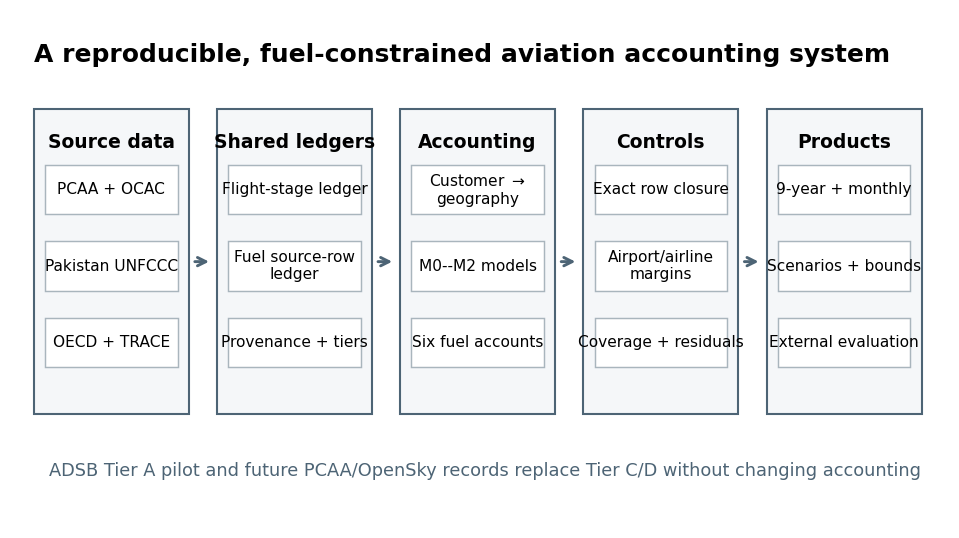
\includegraphics[width=0.94\textwidth]{aviation_framework.png}
\caption{Data sources populate conserved fuel and flight ledgers, from which accounting
products, domestic model estimates and external evaluations are generated.}
\label{fig:framework}
\end{figure*}

\section{Methods}
\label{sec:methods}

\subsection{Conserved customer-to-geography fuel ledger}

Every OCAC record retains its period, customer category, fuel type, reported tonnes, source
file and revision status. It is assigned across six non-overlapping destinations: IPCC
domestic civil aviation ($d$), international bunkers ($i$), military/government 1A5b ($m$),
general aviation ($g$), export/other ($o$) and unresolved residual ($u$). For each source row
$r$,
\begin{equation}
F_r=F_{r,d}+F_{r,i}+F_{r,m}+F_{r,g}+F_{r,o}+F_{r,u}.
\label{eq:rowclosure}
\end{equation}
Closure is asserted before aggregation. Missing evidence increases $F_{r,u}$; it never triggers
a national rescaling.

Three structural mappings test the customer-to-geography boundary. A literal mapping assigns
resident-airline JP-1 to domestic aviation. A movement-share mapping divides it according to
domestic and international flight stages. The central calibrated mapping uses the OECD
resident-carrier share
\begin{equation}
s_d=\frac{E^{\rm OECD}_{\rm resident,domestic}}
{E^{\rm OECD}_{\rm resident,domestic}+E^{\rm OECD}_{\rm resident,intl.from}},
\label{eq:share}
\end{equation}
which is 25.674\% in FY2023--24. Foreign-customer JP-1 is assigned principally to international
bunkers; government aviation JP-1 and JP-8 are military/government candidates; 100LL is a
general-aviation candidate; and government-other JP-1 remains unresolved. Alternative
carrier-specific movement and modelled-fuel shares preserve separate PIA and other-airline
networks while remaining constrained to the same aggregate OECD share. These mappings are
reported as scenarios, not pooled into a confidence interval.

Three definitions are fixed as accounting invariants. PCAA movements are divided by two to
obtain domestic stages because each flight generates a departure and an arrival. Domestic
status requires both endpoints in Pakistan, irrespective of customer or carrier residence.
Domestic greenhouse gases use full-flight fuel; international airport LTO emissions remain a
separate local-air-quality product \citep{ipcc2006energy}.

\subsection{Domestic activity and fuel models}

The aggregate movement model (M0) multiplies domestic stages by a representative distance and
year-varying fleet intensity:
\begin{equation}
E_y=N_y\,\bar d_y\,I_y,
\end{equation}
where $N_y$ is flight stages, $\bar d_y$ mean distance and $I_y$ fuel and emission intensity.
The route-resolved model (M1) replaces the representative stage with an annual origin--
destination matrix constrained to PCAA airport margins, airline departures and routes
documented for FY2023--24. Unsupported movements remain an unallocated residual. Minimum and
maximum feasible distance are solved over the same route graph and control margins.

The route--aircraft model (M2) assigns probabilistic aircraft-family shares by operator and
route and generates phase-resolved synthetic profiles with OpenAP \citep{sun2020openap}.
Operator passengers, cargo and mail constrain central payload; route detour, taxi time and
aircraft assignment remain uncertain. Unsupported aircraft use a separately identified ICAO
factor, while route, operator and endpoint residuals are completed through explicit lower-tier
methods. A common-support comparison applies all three models to the same 17,491 stages before
those residuals are added, preventing model resolution from being confused with coverage.
Synthetic route strata are never labelled as observed flights.

The flight-stage ledger is source-neutral: observed records may replace reconstructed strata
without changing accounting or emissions code. The detailed route optimiser, source tiers,
OpenAP range checks, ADS-B endpoint rules, payload construction and coverage activation gate
are provided in the supplement.

\subsection{Evaluation and comparison design}

OCAC cumulative monthly values are first-differenced and required to reproduce each final
annual source row. OECD records are aggregated to identical July--June windows. For component
$j$ and month or year $t$,
\begin{equation}
R_{t,j}=\frac{F^{\rm OCAC}_{t,j}\,3.16}{E^{\rm OECD}_{t,j}}.
\end{equation}
We compare resident, foreign and combined commercial accounts and calculate the fraction of
opposite component differences that cancels in their total:
\begin{equation}
C=1-\frac{|\Delta_{\rm resident}+\Delta_{\rm foreign}|}
{|\Delta_{\rm resident}|+|\Delta_{\rm foreign}|}.
\end{equation}
Five complete fiscal years support annual comparison and 42 matched months test whether annual
closure is temporally stable.

The central fuel bridge uses OECD's resident share and therefore tests consistency, not
independent accuracy. The strongest gross closure compares OCAC commercial JP-1 with OECD
combined territory aviation. Aggregate movement, route-resolved and route--aircraft models are
compared externally with OECD domestic territory emissions. Pakistan's CRT tests the official
boundary implementation; Climate TRACE tests fiscal-year magnitude and airport ordering but
may share surveillance or performance inputs. PCAA movement, passenger and route constraints
target specific internal failure modes.

Public ADSB.lol and ERA5 experiments remain supporting diagnostics. The former tests whether a
small public trace sample can replace reconstructed stages; the latter tests the sensitivity of
representative OpenAP flight duration to route winds. Neither is expanded into an observed
annual inventory or counted as fuel validation.

\subsection{Parametric and structural uncertainty}

Parametric and structural uncertainty are evaluated separately. The aggregate movement model
retains its legacy activity/fleet representation term. The completed route--aircraft model uses
20,000 flight-stage Monte Carlo draws within each structural configuration. Aircraft family is
shared within operator--route strata, detour across reciprocal routes, taxi time by airport and
carbon conversion globally. Payload is sampled around PCAA passenger, cargo and mail controls.
CH4, N2O and net calorific value enter only the secondary \COe{} result.

Alternative feasible route matrices and unsupported-activity completion methods define a
structural envelope; customer-to-geography mappings remain a separate accounting scenario.
The route--aircraft model does not inherit the aggregate model's $\pm60$\% representation term.
A drop-one variance screen identifies which named variables drive its interval. Automated QA/QC
asserts source-row and monthly closure, route-bound ordering, common support, coverage
completion, phase-fuel closure, movement balance and agreement between generated outputs and
the manuscript. The complete uncertainty register and assertion catalogue are supplementary.

\FloatBarrier
\section{Results}
\label{sec:results}

\subsection{Do the gross fuel and flight accounts agree?}

OCAC commercial JP-1 corresponds to 1940.9 kt \COtwo{} in FY2022--23 and 2032.1 kt in
FY2023--24. These values are respectively 0.16\% and 0.77\% below OECD's combined domestic and
international territory estimates (Table~\ref{tab:two-year}). Agreement in the latest two
years is therefore close at the gross commercial boundary.

\begin{table*}[htbp]
\centering
\footnotesize
\begin{tabular}{@{}lrrrrrrrr@{}}
\toprule
 & \multicolumn{4}{c}{\textbf{FY2022--23}} & \multicolumn{4}{c}{\textbf{FY2023--24}} \\
\cmidrule(lr){2-5}\cmidrule(lr){6-9}
\textbf{Component} & \textbf{OCAC kt fuel} & \textbf{OCAC kt \COtwo{}} & \textbf{OECD kt \COtwo{}} & \textbf{Ratio} &
\textbf{OCAC kt fuel} & \textbf{OCAC kt \COtwo{}} & \textbf{OECD kt \COtwo{}} & \textbf{Ratio} \\
\midrule
Resident carriers & 346.0 & 1093.3 & 841.8 & 1.299 & 359.9 & 1137.4 & 884.3 & 1.286 \\
Foreign carriers & 268.2 & 847.6 & 1102.3 & 0.769 & 283.1 & 894.7 & 1163.5 & 0.769 \\
Combined commercial & 614.2 & 1940.9 & 1944.0 & 0.998 & 643.1 & 2032.1 & 2047.8 & 0.992 \\
\bottomrule
\end{tabular}
\caption{Matched carrier-component comparison. Government fuel is excluded from the
commercial boundary.}
\label{tab:two-year}
\end{table*}

The longer record prevents the two-year result from being treated as universal. Across the
five complete OECD overlaps, the combined OCAC/OECD ratio is 0.908, 0.892, 0.935, 0.998 and
0.992 from FY2019--20 to FY2023--24. The nine-year OCAC series also captures the fall in
commercial JP-1 from 730.7 kt in FY2017--18 to 328.7 kt in FY2020--21 and its subsequent
recovery. Monthly combined MAPE is 7.39\% in FY2022--23 and 6.92\% in FY2023--24. Annual
near-closure is thus reproducible in the latest years, but neither historically invariant nor
the product of twelve identical monthly ratios. Full annual and monthly panels are reported in
the supplement.

\subsection{Does agreement survive component decomposition?}

Here, ``resident customers'' are PIA and other Pakistani-airline fuel purchasers in OCAC,
whereas ``resident carriers'' are Pakistani airlines identified in the OECD flight account.
The foreign comparison follows the equivalent OCAC and OECD groups.

Aggregate agreement does not survive this decomposition. Resident-customer fuel is 29.9\% and 28.6\% above OECD resident-carrier emissions
in FY2022--23 and FY2023--24, whereas foreign-customer fuel is 23.1\% below OECD non-resident
emissions in both years. The opposite differences cancel by 99.4\% and 97.0\%, leaving a small
combined discrepancy (Figure~\ref{fig:offsets}). Monthly resident ratios average 1.301 and
1.288, while foreign ratios average 0.770 and 0.768. The sign of the mismatch therefore
persists across both years and months.

\begin{figure}[htbp]
\centering
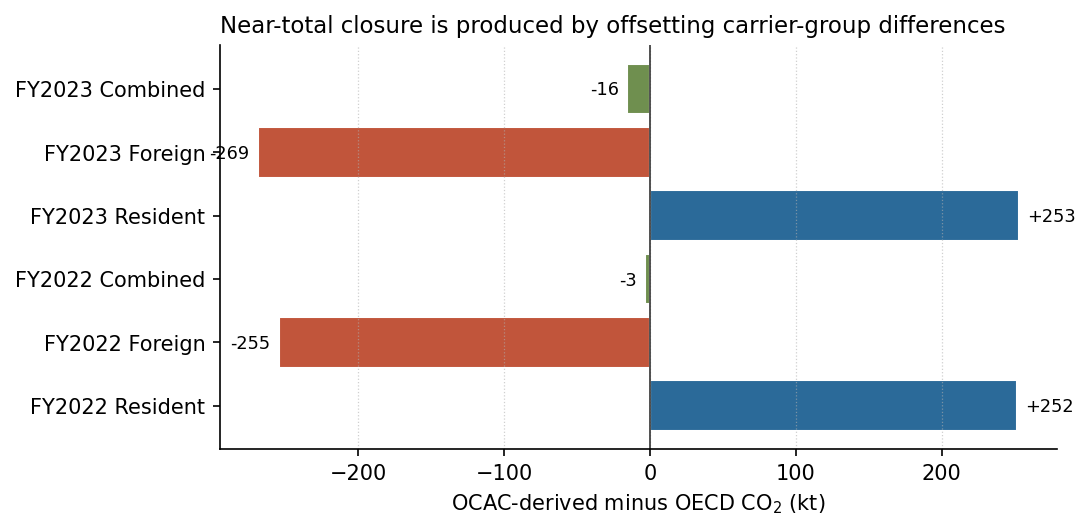
\includegraphics[width=0.92\linewidth]{aviation_component_offsets.png}
\caption{OCAC-derived minus OECD emissions by resident and foreign component. Aggregate
agreement is produced by differences of opposite sign.}
\label{fig:offsets}
\end{figure}

The conserved ledger shows where each reported tonne goes under the central FY2023--24 mapping
(Table~\ref{tab:source-bridge}). PIA and other resident-customer JP-1 contribute 49,760 and
42,649 t to domestic aviation. Their remaining 267,523 t, together with the foreign-customer
row, enters the international-bunker candidate. Government and 100LL streams retain separate
destinations, and an explicit \SI{12282}{\tonne} residual remains unresolved. Every row closes
without using that residual to improve the apparent agreement.

\begin{table*}[htbp]
\centering
\footnotesize
\begin{tabular}{@{}lrrrrrr@{}}
\toprule
\textbf{OCAC source row} & \textbf{Reported t} & \textbf{Domestic} & \textbf{Bunker} &
\textbf{Military} & \textbf{General aviation} & \textbf{Residual} \\
\midrule
Domestic Avi--PIA, JP-1 & 193,813 & 49,760 & 144,053 & --- & --- & --- \\
Domestic Avi--Others, JP-1 & 166,119 & 42,649 & 123,470 & --- & --- & --- \\
Overseas/Foreign Aviation, JP-1 & 283,147 & --- & 283,147 & --- & --- & --- \\
Government Aviation, JP-1 & 2,973 & --- & --- & 2,973 & --- & --- \\
Government Other, JP-1 & 12,282 & --- & --- & --- & --- & 12,282 \\
Government Other, JP-8 & 117,785 & --- & --- & 117,785 & --- & --- \\
All reported 100LL & 4,542 & --- & --- & --- & 4,542 & --- \\
\midrule
\textbf{Total} & \textbf{780,661} & \textbf{92,409} & \textbf{550,670} &
\textbf{120,758} & \textbf{4,542} & \textbf{12,282} \\
\bottomrule
\end{tabular}
\caption{FY2023--24 source-row-conserving fuel bridge under the OECD-calibrated resident
share. Dashes denote zero assignments.}
\label{tab:source-bridge}
\end{table*}

Because customer classes cannot directly supply the domestic boundary, we next compare
alternative estimates of domestic aviation.

\subsection{What does the bridge imply for domestic aviation?}

Using OECD's resident-carrier domestic share assigns 92,409 t of fuel, or 292.0 kt \COtwo{},
to domestic aviation (Table~\ref{tab:bridge-results}). The aggregate movement estimate is
298.9 kt, only 2.3\% higher. Because OECD supplies the partition, this agreement is a
consistency check. Against the independent OECD domestic-territory value of
235.8 kt, the aggregate movement model is 26.8\% higher, the route-resolved model is 14.8\%
higher and the completed route--aircraft model (M2) is 4.7\% higher.

\begin{table}[htbp]
\centering
\scriptsize
\begin{tabular}{@{}lrrr@{}}
\toprule
\textbf{Estimate} & \textbf{Fuel (t)} & \textbf{kt \COtwo{}} & \textbf{Role} \\
\midrule
Aggregate movement (M0) & 94,576 & 298.9 & Unconstrained \\
Route-resolved (M1) & 85,669 & 270.7 & Unconstrained \\
Calibrated fuel bridge & 92,409 & 292.0 & OECD-calibrated \\
Movement-share bridge & 107,555 & 339.9 & Structural \\
Literal customer labels & 359,932 & 1137.4 & Diagnostic \\
Completed route--aircraft model (M2) & 78,139 & 246.9 & Provisional \\
OECD domestic territory & --- & 235.8 & External \\
\bottomrule
\end{tabular}
\caption{FY2023--24 domestic \COtwo{} estimates. Different evidence roles preclude averaging
the rows into one preferred value.}
\label{tab:bridge-results}
\end{table}

The same ordering broadly replicates in FY2022--23: aggregate movement fuel is 101,196 t,
route-resolved fuel 90,446 t, the calibrated bridge 94,314 t and OECD domestic territory
237.2 kt \COtwo{}. Including CH4 and N2O gives
\SI{0.294}{\mega\tonne} \COe{} for the FY2023--24 bridge, compared with 0.301 Mt for the
aggregate movement model. The central bridge also assigns 550,670 t of commercial JP-1 to
full-flight international bunkers, or \SI{1.740}{\mega\tonne} \COtwo{}. That quantity is
distinct from the 210.4 kt international LTO estimate at Pakistani airports. The
non-commercial fuel the bridge identifies is now priced too, as memo rows beside the
bunkers: 120,758~t of military and government jet fuel (\SI{381.6}{\giga\gram}
\COtwo{}), 4,542~t of 100LL general aviation (\SI{14.1}{\giga\gram}) and 12,282~t of
unresolved government JP-1 (\SI{38.8}{\giga\gram})---together about
\SI{0.434}{\mega\tonne}, larger than the reported domestic sector, outside the
1.A.3.a total because IPCC books military aviation under 1A5b and no record attributes
the activity; the scope choice is priced against the national total as three
independent configurations, one per fuel evidence class, and the same
streams ship as a first-class OBSERVED-UNALLOCATED ACCOUNT
(\texttt{outputs/aviation\_unallocated\_fuel\_fy2023\_24.csv}: each identified tonne
with a closed evidence class, its disposition, and the record that would close
it), so booked-outside-the-boundary can never read as absent, because military
attribution, general-aviation activity and the bridge residual are separate
questions: \emph{military\_government\_in\_scope} (\num{445.33702}~Mt),
\emph{general\_aviation\_in\_scope} (\num{444.96950}~Mt) and
\emph{unresolved\_jp1\_in\_scope} (\num{444.99423}~Mt), each against the
\num{444.95542} reference.

\begin{figure}[htbp]
\centering
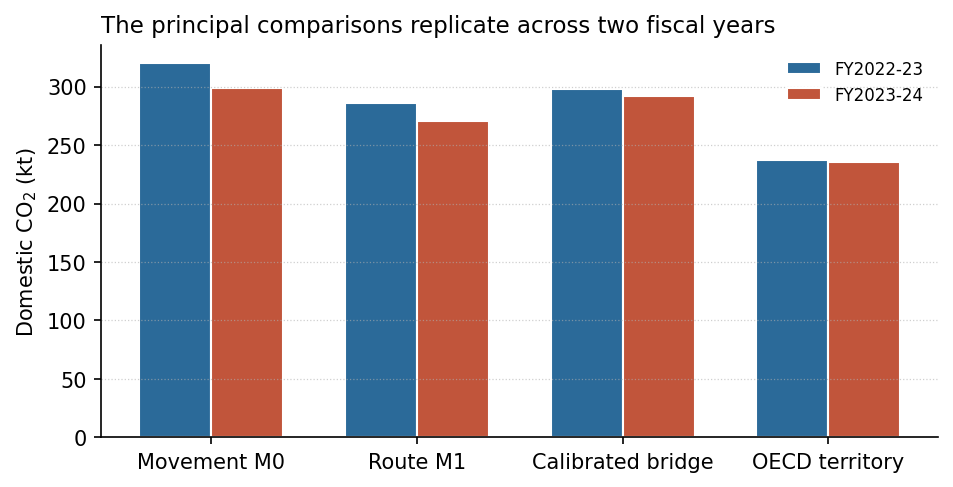
\includegraphics[width=\linewidth]{aviation_two_year.png}
\caption{Two-year comparison of aggregate movement, route-resolved, calibrated-bridge and
OECD domestic estimates.}
\label{fig:domestic-comparison}
\end{figure}

\begin{figure*}[htbp]
\centering
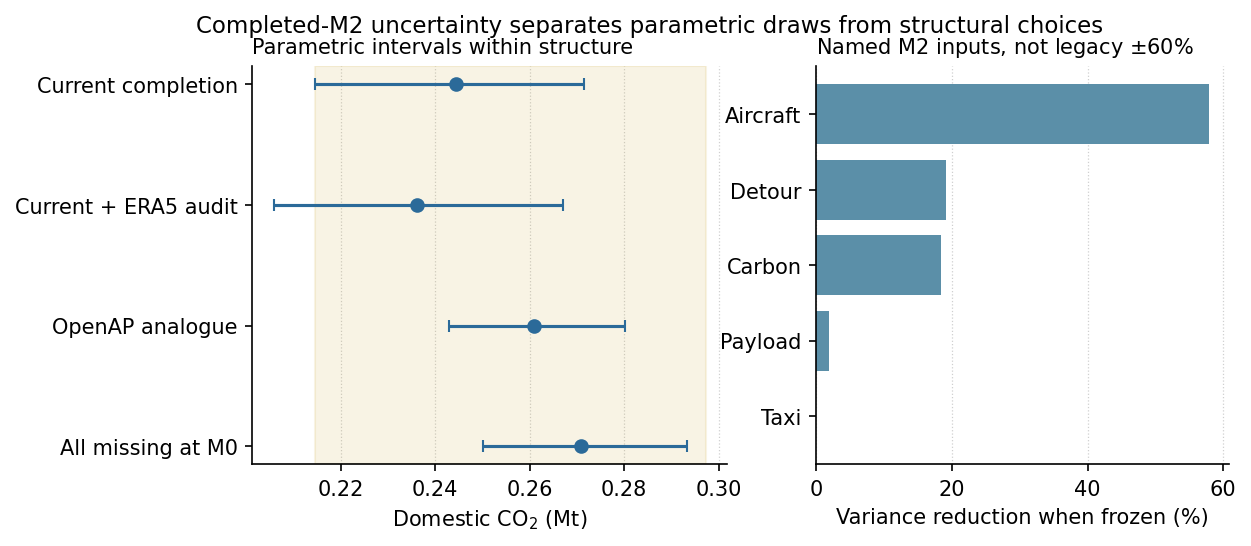
\includegraphics[width=0.78\textwidth]{aviation_m2_uncertainty.png}
\caption{Route--aircraft Monte Carlo intervals, structural envelope and drop-one variance
diagnostics for the completed route--aircraft model.}
\label{fig:route-aircraft-uncertainty}
\end{figure*}

Carrier-specific scenarios change attribution within the resident rows but not the calibrated
total. After constraining separate PIA and other-carrier movement shares to the same aggregate,
their domestic shares are 20.0\% and 32.2\%. Partial modelled-fuel shares are not used because
only 27.9\% of resident international departures are reconstructed.

\subsection{Are the findings supported by other evidence?}

Pakistan's official calendar-2022 CRT reports 654.1 kt domestic and 163.5 kt international
aviation \COtwo{}, compared with matched OECD values of 232.9 and 1713.3 kt
(Figure~\ref{fig:official}a). The official workbook applies an explicit 80\% domestic and 20\%
international fuel distribution, labels the activity aviation gasoline and marks jet kerosene
not estimated. Its domestic and international ratios to OECD are therefore 2.808 and 0.095.
The reported allocation is not consistent with the petroleum and flight-geography evidence
examined here, and its institutional derivation could not be reconstructed. The supplement
provides the workbook hash and cell-level audit.

Climate TRACE gives 255.9 kt domestic and 1950.9 kt international \COtwo{} for FY2023--24,
8.5\% and 7.7\% above OECD. Its airport ordering is strongly associated with PCAA activity:
Spearman's $\rho=0.971$ across 16 domestic airports and 0.948 across 11 international airports
(Figure~\ref{fig:official}b). This supports the broad spatial pattern, not independent fuel-burn
accuracy.

\begin{figure*}[htbp]
\centering
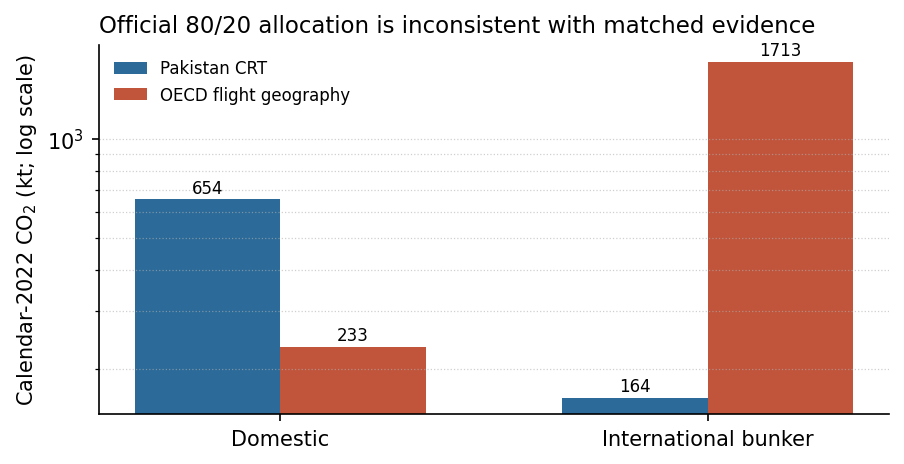
\includegraphics[width=0.43\textwidth]{aviation_official_reporting.png}\hfill
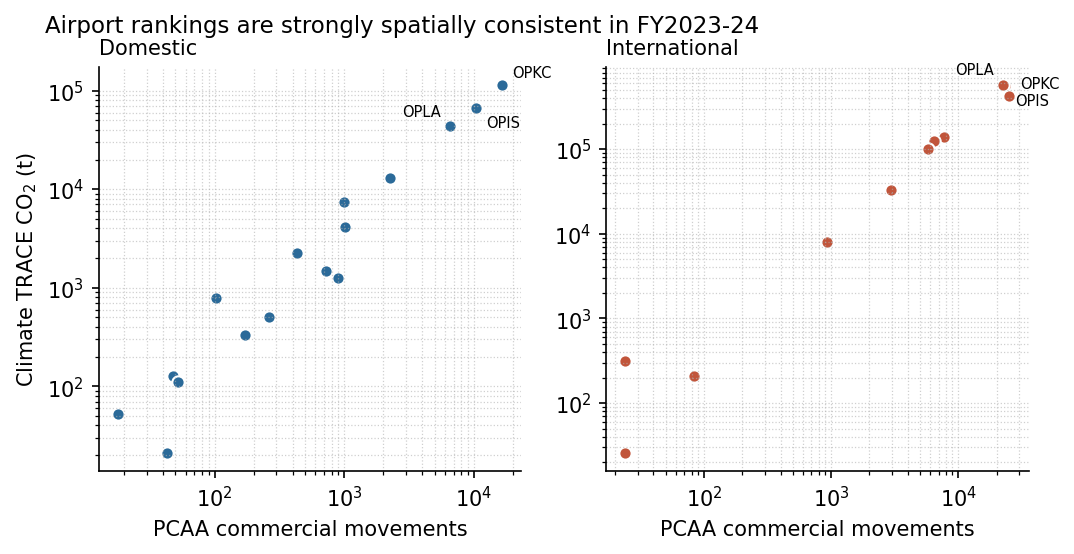
\includegraphics[width=0.54\textwidth]{aviation_climatetrace_airports.png}
\caption{External diagnostics. (a) Pakistan's calendar-2022 CRT categories versus matched
OECD flight-geography estimates. (b) FY2023--24 PCAA airport movements versus Climate TRACE
airport \COtwo{}.}
\label{fig:official}
\end{figure*}

\subsection{What remains uncertain?}

The documented route graph allocates 20,098 of 20,300 domestic stages. Conditional on PCAA
margins and supported links, its minimum, central and maximum mean distances are 485.2, 486.5
and 503.0 nmi. On identical 17,491-stage support, aggregate factors produce 81,490 t fuel,
route-specific distance 76,102 t and route--aircraft profiles 73,439 t. Route resolution lowers
fuel by 6.6\% and the aircraft/performance layer by a further 3.5\%. Explicit completion of
unsupported aircraft and unallocated activity yields 78,139 t.

For the central structure, the route--aircraft Monte Carlo gives mean domestic emissions of
0.244 Mt \COtwo{} from 20,000 draws
(95\% interval 0.215--0.272 Mt). Alternative route graphs and completion methods widen the
endpoint envelope to 0.215--0.297 Mt. Aircraft assignment reduces simulated variance by
57.9\% when frozen, followed by detour (19.2\%) and carbon conversion (18.4\%); these drop-one
responses are non-additive. The remaining uncertainty is consequently tied to identifiable
flight-stage quantities rather than the aggregate model's umbrella representation term.

Supplementary tests support the treatment of the completed route--aircraft model. A physical
range assertion identified and corrected an OpenAP distance-unit mismatch, after which the
common-support performance difference fell from 39.4\% to 3.5\%. Sampled ERA5 winds changed
representative fuel by $-3.9$\% on average. A four-day ADSB.lol pilot provided no usable
Pakistan-airport stages despite passing synthetic and same-archive positive controls;
reconstructed activity is therefore retained rather than expanded from inadequate
observations.

\FloatBarrier
\section{Discussion}
\label{sec:discussion}

The central result is not simply that two national totals agree. In the latest two fiscal
years, OCAC commercial fuel and OECD combined territory aviation differ by less than 1\%, but
resident and foreign components differ by about $+29$\% and $-23$\%. The signs persist in the
monthly record, and the five-year combined ratio ranges from 0.892 to 0.998. Aggregate closure
is therefore a useful check on the gross boundary, but it cannot establish that customer
categories have been assigned correctly. Indeed, the closer the cancellation, the easier it
is for a component error to disappear from the national total.

The conserved ledger changes how that evidence is interpreted. It prevents a customer label
from being promoted directly to an IPCC category, preserves the international counterpart of
every domestic assignment and leaves unsupported fuel as a statistical discrepancy. It also
separates four quantities that serve different users: domestic aviation under the IPCC flight
boundary, full-flight international bunkers, resident-carrier emissions and emissions located
physically over Pakistan. A single fuel-sales label cannot represent all four.

Pakistan's official submission demonstrates the policy relevance. Its 80/20 distribution
produces domestic and international estimates on opposite sides of the flight-geography
evidence by factors of 2.81 and 0.095. The official values should not be dismissed merely
because they differ from OECD, which is itself modelled. However, the aviation-gasoline label,
the absence of estimated jet kerosene and the inability to reconstruct the allocation from
public documentation mean that the split warrants institutional review. The appropriate next
step is to reconcile the CRT activity data with OCAC jet-fuel rows and actual domestic and
international flight stages, rather than replace one opaque percentage with another.

The hierarchy of domestic estimates localises the remaining scientific uncertainty. Across the
complete inventory, replacing the 550-nmi representative stage with the constrained route
matrix lowers fuel by 9.4\%. On the identical 17,491-stage subset used for the resolution
experiment, the corresponding reduction is 6.6\%. Adding aircraft-specific OpenAP profiles on
that common support lowers fuel by a further 3.5\% after a physical range check corrected the
earlier software interface error. The route--aircraft Monte Carlo mean of 0.244 Mt \COtwo{} is
close to OECD's 0.236 Mt, but this is model-to-model agreement, not observed block-fuel
validation. Its
probabilistic and structural ranges identify aircraft assignment, detour and completion rules
as actionable uncertainties. PCAA passenger, cargo and mail data already constrain payload;
registrations, route-complete international activity and airline block fuel would test the
remaining assumptions directly.

The external comparisons have deliberately different roles. Climate TRACE reproduces the
airport ranking and broadly agrees on fiscal-year magnitude, but may share flight-surveillance
and performance inputs with OECD or a future ADS-B implementation. The negative ADSB.lol pilot
does not undermine the accounting result: positive controls show that the adapter works, while
the Pakistan sample does not meet the coverage gate. Observed flight records would replace one
input tier and test the present estimates; they are not required to make source-row conservation
or component cancellation valid.

The approach is transferable wherever petroleum statistics follow purchasers while greenhouse-
gas inventories follow flight geography. The essential requirements are modest: preserve each
fuel source row, distinguish customer from operator and endpoints, disclose the role and shared
inputs of every comparison, and report structural mappings separately from parametric
uncertainty. More detailed trajectory or aircraft models then improve a defined layer of the
account rather than silently changing its boundary.

\section{Limitations}
\label{sec:limitations}

The central domestic fuel partition is calibrated with OECD's resident-carrier share. It is
therefore not independently validated by its subsequent proximity to OECD or to the aggregate
movement estimate. The route reconstruction covers domestic activity well but only 27.9\% of
resident international departures, so it cannot yet replace that share. OCAC customer rows
also lack airport- and operator-specific uplift detail, and the meaning of government-other
JP-1 remains unresolved.

The flight-stage layer is predominantly reconstructed. Route evidence and PCAA margins bound
distance, while passengers, cargo and mail constrain payload, but aircraft registrations,
flight-specific mass, detour, taxi time, weather and block fuel are not observed. The public
ADSB.lol pilot covers only four days and should not be generalised to all ADS-B providers. The
extended fuel ledger is not an observed annual route--aircraft inventory: detailed route
and fleet reconstruction is anchored to FY2023--24. FY2024--25 airport movements are own-year activity, while its aircraft composition is explicitly carried from the reference era.

OECD and Climate TRACE are modelled products rather than direct fuel measurements, and their
surveillance or performance inputs may overlap. The CRT is an official comparator, not ground
truth; the public workbook does not reveal the institutional derivation of its 80/20 split.
Monthly OCAC values are differences of cumulative reports, so revisions can shift apparent
fuel between adjacent months even when annual closure is exact.

Finally, general aviation, training and military activity are not separated operationally.
The spatial product is limited to airport LTO: no province, district or route--altitude cruise
allocation is inferred from synthetic trajectories. The admitted LTO pollutant estimate uses
representative engines and omits observed taxi times, APU, ground support, non-exhaust sources
and near-airport measurements; it is not a complete airport micro-inventory.

\section{Conclusion}
\label{sec:conclusion}

Pakistan's commercial aviation fuel and OECD flight estimates nearly close in aggregate in the
latest two fiscal years, but that agreement is produced by large component differences of
opposite sign. In FY2023--24 resident-customer fuel is 28.6\% above the resident-carrier
estimate, foreign-customer fuel is 23.1\% below the non-resident estimate and 97\% of the
discrepancy cancels. Pakistan's official 80/20 allocation produces a still larger domestic--
international mismatch. National agreement is therefore a necessary gross check, not evidence
that purchaser categories implement flight geography.

The national inventory carries the aggregate movement model's \SI{0.301}{\mega\tonne}
\COe{} as domestic aviation's figure. The central bridge assigns 0.292 Mt \COtwo{};
aggregate-movement, route-resolved and completed route--aircraft estimates are 0.299,
0.271 and 0.247 Mt as \COtwo{}; the route--aircraft Monte Carlo mean is 0.244 Mt with a
95\% interval of 0.215--0.272 Mt. These estimates place domestic aviation in a common broad range while showing
that customer partition, aircraft assignment and incomplete international coverage remain the
most consequential uncertainties.

The general contribution is an accounting method rather than one assertedly final national
number. Every fuel source row is conserved, residuals remain explicit, evidence roles are
declared and structural mappings are kept outside parametric confidence intervals. Observed
flight stages and detailed uplift records can now test and replace
provisional inputs without changing those rules.

\FloatBarrier

\section*{Code and data availability}
The calculation engine, normalized activity data, source hashes and every output quoted here
are version-controlled in the inventory repository
(\url{https://github.com/RehanAhmad13/pakistan-emissions-sectors}). The supplement gives the full reproduction sequence, source hashes,
uncertainty register and assertion catalogue. The multi-gigabyte ADSB.lol cache is not
redistributed under the ODbL; only aggregate pilot diagnostics are released. Manuscript values
are checked against generated outputs.

\bibliographystyle{elsarticle-harv}
\bibliography{../../paper_common/references}

\end{document}
